\documentclass{beamer}
\usepackage{graphicx}
\usepackage[export]{adjustbox}
\usepackage{amsmath}
\usepackage{fourier}

\usepackage{pgfpages}
\setbeameroption{show notes}
\setbeameroption{show notes on second screen=left}
\begin{document}
\title{Introduction to Software Security}
\subtitle{Understanding the core concepts}
\author{Bruce Ricard, VMware}
\date{\today}

\frame{\titlepage}

\frame{\
  \frametitle{Agenda}
  \tableofcontents
}

\frame{
  \frametitle{Preface}

  This presentation attempts to present a few important concepts
  related to software security.
  \\~\

  We don't expect the attendees to have any particular knowledge about
  math or cryptography or computer science.
  \\~\

  We'll go slowly and not dig too deep into any topic.
}

\section{Cryptography}
\subsection{Historical context}
\frame{
  \frametitle{Cryptography}
  \framesubtitle{A little history}

  \note{The romans started encrypting their communications so that
    their ennemies wouldn't know what their plans were. And that is
    also why we encrypt.

    Cryptography is the science of encrypting and decrypting data to
    protect communication channels.

    NB: cryptography doesn't need computers.}

  Caesar cipher
  \pause
  \begin{figure}
    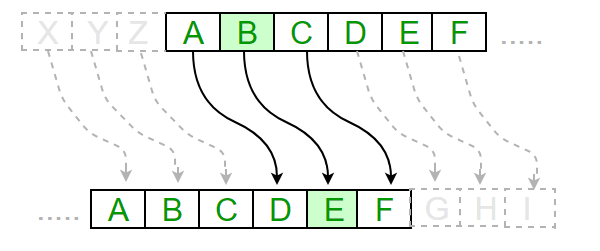
\includegraphics[scale=0.3]{images/caesar_cipher.png}
  \end{figure}

  Example: $``I LOVE CRYPTOGRAPHY'' \rightarrow
  ``L ORYH FUBSWRJUDSKB''$

  \pause

  \vspace{\baselineskip}
  Symmetric(-Key) Cryptography
}

\subsection{Theory}
\frame{
  \frametitle{Cryptography}
  \framesubtitle{Vocabulary}

  Symmetric Cryptography diagram: \\~\

  $$ plain text \xrightarrow[key]{encryption}
  ciphertext \xrightarrow[key]{decryption} plain text $$

  \note{you'll also see ``clear text''}
}

\frame{
  \frametitle{Cryptography}
  \framesubtitle{Symmetric cryptosystem examples}

  \note{Cryptosystem: set of algorithms used to implement a particular
    ``security service''}

  \note{You can improve a lot on the Caesar cipher by chosing a random
    permutation of the letter instead of just always adding the same
    number}

  \begin{itemize}
  \item Caesar cipher
  \item Data Encryption Standard (DES) (1975)
  \item Advanced Encryption Standard (AES) (1998)
  \end{itemize}
}

\subsection{Practice}
\frame{
  \frametitle{Cryptography}
  \framesubtitle{Issues with symmetric cryptography}

  \begin{itemize}
  \item Sharing key with other parties
  \item Different key for every party
  \end{itemize}
  \pause
  \medskip
  $\rightarrow$ Public Key cryptography
}

\frame{
  \frametitle{Cryptography}
  \framesubtitle{Modular arithmetic}

  Very common in cryptography

  \note{Z is the set of integers\\}

  \note{pronounced ``zee over twelve zee''}

  In $\mathbb{Z}/12\mathbb{Z}$ (numbers modulo 12)

  $ 8 + 7 = 15 = 12 + 3 = 3 \pmod{12}$

}


\frame{
  \frametitle{Cryptography}
  \framesubtitle{Public key cryptography}

  One way functions
  \pause

  In $\mathbb{Z}/100\mathbb{Z}$ (numbers modulo 100)

  $$ f : n \mapsto n^2 $$

  $f(41) = 41^2 = 1681 = 16 * 100 + 81 = 81 \pmod{100}$

  \note {This function is very easy to calculate, but it is also very hard to find all numbers x such that f(x) = 81, by opposition to the integers for example}
}

\frame{
  \frametitle{Cryptography}
  \framesubtitle{Hashing}

  Cryptographic versus non-cryptographic hashing.
  \\~\
  First example of one way functions.
  \\~\

  \note<1> {hashes are non-injective, hence these one way functions don't
    even have an inverse}

  \pause

  Words you might hear: salt, pepper, nonce
  \\~\

  \note<2> {These things all refer to strings that are appended to to
    the plain text before encryption in order to make attacks harder}

  \pause

  Examples:
  \begin{itemize}
  \item MD5
  \item SHA family
    \pause
  \item bcrypt
  \end{itemize}
}

\frame{
  \frametitle{Cryptography}
  \framesubtitle{Public key cryptography}

  RSA (Rivest--Shamir--Adleman 1977)
  \begin{itemize}
  \item Public Key: modulo $n$, number $e$
  \item Private Key: number $d$
  \end{itemize}
  Such as for any $x$, number modulo $n$:
  $$ x^{e.d} = x \pmod{n} $$

  \pause

  Encryption: $ p \mapsto p^e $ ;
  Decryption: $ c \mapsto c^d $
}

\frame{
  \frametitle{Not Cryptography}
  \framesubtitle{Encoding}

  A representation of data.

  \note {In colloquial use, the term "code" is often used to mean any method
    of encryption or concealment of meaning.}

  Beware of the word ``code'' from the English language:
  \begin{itemize}
  \item Code to enter the building
  \item Passcode to unlock your phone or computer
  \item Codenames
  \end{itemize}

  \pause
  Examples:
  \begin{itemize}
  \item ASCII
  \item UTF-8
  \item Base 64
  \item URL encoding
    \pause
  \item Written English
  \item Drawings
  \item Radio waves
  \item Sound waves carrying spoken languages
  \end{itemize}

  In software: ``character encoding''

  \note{Encoding: write the data so that it can be understood by everybody
  else.

  Encrypting: write the data so that almost nobody can undertand what
  it means

  I understand the word ``encoding'' can be quite confusing since in
  contains the word ``code'' in it, but remember that it has nothing
  to do with cryprography.

  One could say a cipher is a particular kind of encoding of some
  information.}

  \note {For example, kubernetes says they encode secrets by default
    using base 64 encoding}
}



\frame{
  \frametitle{Cryptography}
  \framesubtitle{Issues with public key cryptography}

  Slow, can only encrypt little data
  (by design -- one-way functions)

  Anybody can encrypt data: no more sender validation

  \vspace{\baselineskip}
  $\rightarrow$ Digital Signatures
}

\frame{
  \frametitle{Cryptography}
  \framesubtitle{Signing / Validating}

  Use Public Key Cryptography to sign: but ``encrypt'' with private
  key.

  \pause

  \begin{itemize}
  \item Public Key: modulo $n$, number $e$
  \item Private Key: number $d$
  \end{itemize}
  Such as for any $x$, number modulo $n$:
  $$ x^{e.d} = x \pmod{n} $$

  Encryption: $ p \mapsto p^e $ ;
  Decryption: $ c \mapsto c^d $

  \note<2>{To encrypt, one uses the other party's public key}

  \pause

  \note<3>{To sign,
    one uses their own private key\\}
  \note<3>{To validate the signature, you need to also have the plain
    text\\}

  Signing: $ p \mapsto p^d $ ;
  Validation: $ s \mapsto s^e $
}

\frame{
  \frametitle{Cryptography}
  \framesubtitle{Summary}

  \begin{itemize}
  \item Symmetric Cryptography:
    \begin{itemize}
    \item uses a single \textit{key}
    \item fast
    \item requires key exchange
    \end{itemize}
  \item Public key (Asymmetric) Cryptography:
    \begin{itemize}
    \item uses a key pair: a \textit{public key} and a \textit{private key}
    \item slow
    \item doesn't require key exchange
    \item can be used to sign
    \end{itemize}
  \end{itemize}
}


\frame{
  \frametitle{Crytograpy}
  \frametitle{What can we do with this?}

  \begin{itemize}
  \item Encrypt data so that it can only be read by entity with decoding key
  \item Making sure that the right entity has the decoding key
  \end{itemize}

  \pause
  \begin{itemize}
  \item Encrypt AES key with RSA
  \item Sign RSA public keys / owner by trusted party \pause : certificates
  \end{itemize}
}

\frame{
  \frametitle{Cryptography}

  Questions?
}

\frame{
  \frametitle{Cryptography}
  \framesubtitle{Issues with signatures}

  Signing proves that you own the Key Pair.

  \pause
  \vspace{\baselineskip}

  But how do you prove who you actually are?

  \pause
  \vspace{\baselineskip}

  $\rightarrow$ Certificates
}

\section{Communicating safely using cryptography}
\subsection{Certificates}
\frame{
  \frametitle{Certificates}
  \framesubtitle{Examples}

  \begin{itemize}
  \item birth certificate
  \item marriage certificate
  \item state ID
  \item driver's license
  \item international passport
  \end{itemize}

  What do they have in common?
}

\frame{
  \frametitle{ID cards}
  \framesubtitle{why do we use them?}

  Why do we have IDs?

  \pause

  Proof for information

  \pause

  The 3 main categories on an ID card?

  \pause

  \begin{itemize}
  \item Proof that it belongs to a certain entity \& method for
    anybody to validate that
  \item Proof that it was emitted by a trusted authority
  \item Data the entity wants certified
  \end{itemize}

  \pause

  Authorities in place:
  \begin{itemize}
  \item State government: Certificate Authority (CA)
  \item DMV: Registration Authority (RA)
  \item TSA agent with ultraviolet light: Validation Authority (VA)
  \end{itemize}
}

\subsubsection{X.509}
\frame{
  \frametitle{Digital Certificates}
  \framesubtitle{identity}

  electronic-IDs for software \pause :

  \begin{itemize}
  \item X.509
    \begin{itemize}
    \item Name / URL
    \item trusted signature
    \item public key
    \end{itemize}
  \end{itemize}

  Formalized concepts of CA and RA.
}

\frame{
  \frametitle{Certificates}

  Questions?
}

\subsection{PKI}
\frame{
  \frametitle{PKI}
  \framesubtitle{Public Key Infrastructure}

  A PKI consists of:
  \begin{itemize}
  \item A certificate authority (CA)
  \item A registration authority (RA)
  \item A central directory (for key storage)
  \item A certificate management system (e.g. who can access the stored keys)
  \item A certificate policy (stating the PKI's requirements concerning its procedures.
    Its purpose is to allow outsiders to analyze the PKI's trustworthiness.)
  \end{itemize}
}

\subsection{SSL / TLS}
\frame{
  \frametitle{SSL / TLS}
  \framesubtitle{TLS - Transport Layer Security}
  \begin{itemize}
  \item Cryptographic protocol for safe communication over computer network
    \pause
  \item Previously: SSL - Secure Sockets Layer (1994)
    \pause
  \item TLS 1.0 (1999)
  \item Now TLS 1.3 (2018)
  \end{itemize}
}


\frame{
  \frametitle{SSL / TLS}
  \framesubtitle{TLS handshake (simplified)}

  \pause
  \begin{enumerate}
  \item Client makes $https$ call to server: initiates TLS handshake
  \item Server sends its $x509$ certificate
  \item Client validates certificate signature against CA
  \item Client validates certificate hostname and gets public key $p$
  \item Client generates random string to be symetric private key $k$
  \item Client encrypt $k$ with server's public key $p$, and sends it to the server
  \item Server decrypts encoded key with its private key
  \end{enumerate}

  \pause
  End of handshake:
  \begin{itemize}
  \item client validated identity of server
  \item both parties have secure secret key for encrypted private communication
  \end{itemize}

  \pause
  Server and client will now communicate by encrypting and decrypting any data sent
  over the wire with their private key, using a symetric algorithm like AES.
}

\frame{
  \frametitle{How does TLS work?}
  \framesubtitle{Why is it secure?}

  \begin{itemize}
  \item encrypts data
  \item makes sure the right entity can decrypt
  \end{itemize}
}

\frame{
  \frametitle{TLS}
  \framesubtitle{What is --skip-ssl-validation?}

  Or in the browser ``This page in not secure...''
  \pause

  Not encrypting data? \pause Yes it is.
  Not validating identity: self-signed certificate.
}

\frame{
  \frametitle{mTLS}
  \framesubtitle{mutual TLS}

  \begin{itemize}
  \item With TLS, client validates identity of server. Client doesn't authenticate.
  \item Most websites use username/password for client authentication.
  \item mTLS can be done with username/password: we'll look at certificate based mTLS
  \end{itemize}

  \pause
  Not MTLS
}

\frame{
  \frametitle{mTLS}
  \framesubtitle{mTLS handshake (simplified)}

  \begin{enumerate}
  \item server sends its certificate to client
  \item client validates certificate signature and hostname
  \item client sends its certificate to server
  \item server validates certificate signature
  \item server generates random key to use as private symmetric key and sends
    to client
  \end{enumerate}

  \pause

  Both entities validated that the other party is trustworthy
}

\frame{
  \frametitle{TLS}
  \framesubtitle{TLS termination}

  \begin{itemize}
  \item TLS termination proxy
  \item TLS forward proxy
  \end{itemize}
  \pause
  CF does mostly TLS forward proxy, calls it TLS termination proxy
}


\frame{
  \frametitle{TLS}

  Questions?
}

\frame{
 \frametitle{The end}
 \framesubtitle{}

 
\includegraphics[scale=0.3]{images/keep-calm-and-encrypt-everything.jpg}
 Thank you!
}

\end{document}
